\documentclass{beamer}
\usetheme{Warsaw}
\usepackage{fancybox,graphics}

\title{Delving into Corsi: Building predictors for shot attempts in hockey}
\author{Patrick Rooney}

\date{November 6, 2017}

\begin{document}
\begin{frame}
        \titlepage
\end{frame}

\begin{frame}
        \frametitle{Motivation}
	A player's Corsi-for percentage in hockey is a measure of how many shots his team attempts while he is on the ice: \\
	\[ CF\% ( X) = \frac{\text{shot attempts for X's team while X on-ice}}{\text{shot attempts for both team while X on-ice}} \]

	\vspace{0.1in}
	Note: Shot-attempt = shot on goal OR shot missed / blocked \\
	
	
	\vspace{0.1in}
	Questions: 
	\begin{itemize}
	\item Can we predict shot-attempts using the $CF\%$ statistic?
	\item Can we build a $better$ predictor, using all shot attempt data?
	\item Most importantly: is the $CF\%$ a good measure of how a player influences shot attempts?
	\end{itemize} 
        
\end{frame}



\begin{frame}
          \frametitle{Our Data Set }

Main data set:
	\begin{itemize}
	\item All 1,230 regular-season games in the 2015-2016 NHL season
	\item 136,540 shot attempts (of which 66,601 were on goal, and 6,565 were goals)
	\item 900 players (no goalies). Player on home-ice treated differently then on away-ice (home-ice advantage is real!)
	\end{itemize} 
Additional data:
	\begin{itemize}
	\item Salaries of all players
	\item Average time-on-ice per game for all players
	\end{itemize} 


\end{frame}

\begin{frame}
          \frametitle{Home-ice advantage}

Home-ice advantage is worth on average 0.198 goals/game, and 3.582 shot attempts/game.\\
\vspace{0.2in}

        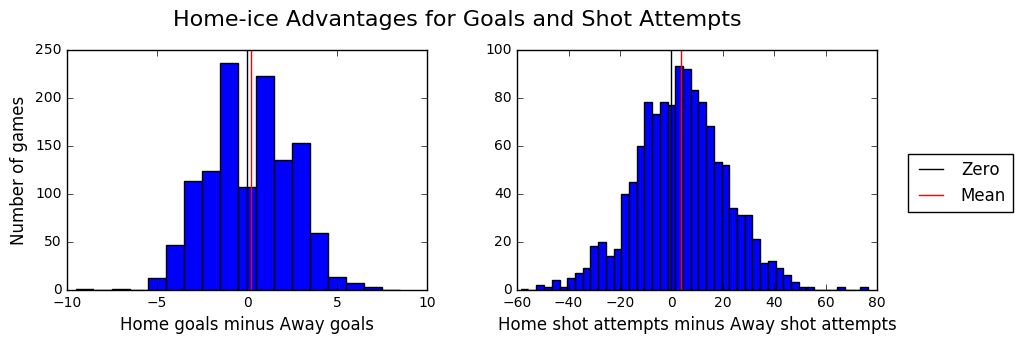
\includegraphics[height=1.5in]{home_ice.png}


\end{frame}


\begin{frame}
          \frametitle{Distribution of Shot-attempts}
          
Studying shot-attempts instead of shots on goal gives us bigger sample size.
          
        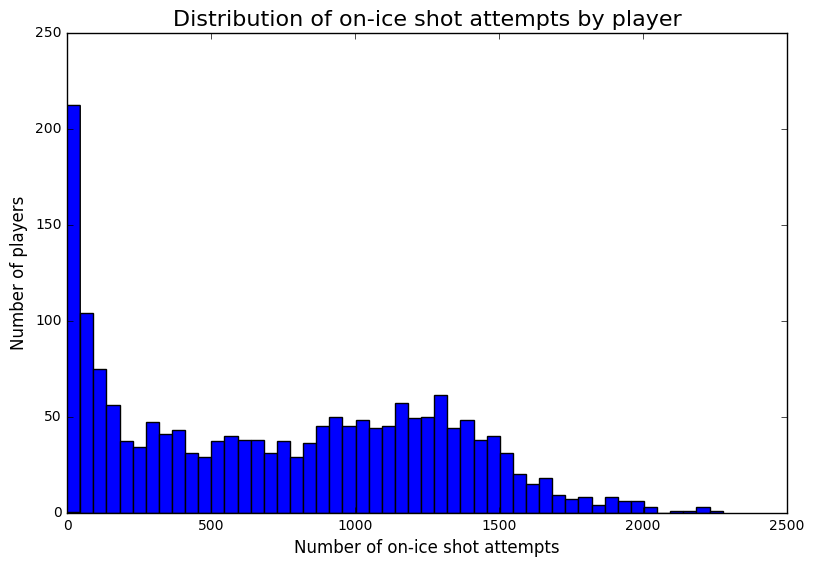
\includegraphics[height=2.4in]{shot_dist.png}

\end{frame}


\begin{frame}
          \frametitle{Predictors}

	We want to build a shot-attempt predictor, based on data from the 2015-2016 NHL season. There were 136,500 attempted shots in this season, and a total of 900 players (excluding goalies). We built three different algorithms, using three different 
	
	\begin{enumerate}
	\item A logistic regressor using only six features: the cumulative $CF\%$ of home and away players, the average salaries, and the average playing time.
	\item A logistic regressor using individual 1,800 binary features. Each player has two features: whether he is on-ice at home, or away. 
	\item A random forest algorithm using the 1above,800 features.
	\end{enumerate}

\end{frame}

\begin{frame}
          \frametitle{Crude Logistic Regressor}

\end{frame}

\begin{frame}
          \frametitle{Sensitive Logistic Regressor}

\end{frame}

\begin{frame}
          \frametitle{Random Forest Predictor}

\end{frame}


\begin{frame}
          \frametitle{Findings}

\end{frame}

%\section{Open Quantum Systems}
%\subsection*{Open vs. Closed Systems}
%\begin{frame}
%           \frametitle{Open vs. Closed Systems}
%
%        \textbf{Closed Quantum System:}
%                \pause
%                \begin{itemize}
%                      \item A state is a ray in a complex Hilbert space $|\psi(t)\rangle$,\\
%                      \pause
%                      or, alternatively, a vector with norm one.\pause 
%                      \item The probability that the state is in some other state $|\phi\rangle$ is given by the modulus-squared of the inner product:
%                      \begin{center} $|\langle\phi|\psi(t)\rangle|^2$ \end{center}
%                      \pause
%                      \item To conserve norm (\textit{i.e.} probability), states at different times are connected by a unitary operator: \\
%                        \begin{center}  $|\psi(t_2)\rangle=U(t_1,t_2)|\psi(t_1)\rangle$   \end{center} \pause
%                      \item The Schrodinger equation is essentially the derivative of norm conservation: \\
%                        \begin{center}   $\frac{d}{dt}|\psi(t)\rangle = -iH |\psi(t)\rangle$   \end{center}   
%                        where $H$ is the self-adjoint Hamiltonian operator.
%                \end{itemize}
%\end{frame}
%
%\begin{frame}
%\frametitle{Open vs. Closed Systems}
%        \textbf{Open Quantum System:}
%                \pause
%                \begin{itemize}
%                        \item A state is an operator $\rho(t)$ on the Hilbert space, called the density matrix or density operator. \pause
%                        \item The eigenvalues of $\rho$ are interpreted as the probabilities the system is in the associated eigenvector. \pause
%                        \item For this interpretation to work, $\rho(t)$ must be positive semi-definite, with trace one.  \pause
%                        \item A density matrix that corresponds to a vector in the closed quantum system is a rank-one operator
%                        \begin{center} $|\psi\rangle\langle\psi|$ \end{center}
%                            and is called a pure state.   \pause
%                        \item The analog of the Schrodinger equation is the von Neumann equation
%                        \begin{center} $\frac{d}{dt}\rho(t) = [-iH , \rho(t) ]   $  \end{center}
%                   
%
%                \end{itemize}
%\end{frame}
%
%
%\subsection*{Lindblad Dissipation}
%\begin{frame}
%\frametitle{Lindblad Dissipation}
%
%von Neumann equation assumes zero interaction with environment. \pause \\
%\vskip5pt
%
%To add dissipation that is \\
%\begin{enumerate} \item Markovian \pause and \item time-inhomogeneous: \pause \end{enumerate}
%
% \begin{block}{\textbf{Lindblad-Kossakowski equation}}
%
%\[  \frac{d}{dt}\rho = [-iH, \rho] + \sum_{i,j=1}^{n^2-1} a_{ij} \left( L_{i} \rho L^\dagger_{j} - \frac{1}{2}\{L^\dagger_{j}L_{i}, \rho  \} \right)    \] \pause
%\begin{itemize}
%\item The operators $\{L_{i}\}$ are an orthnormal basis for traceless operators on the Hilbert space.\pause
%\item The coefficients $a_{ij}$ form a positive semi-definite matrix $A$.
%\end{itemize}
%\end{block}
%
%\end{frame}
%
%\section{Projection onto the Eigenvalue Space}
%
%\subsection*{Limitations of Hamiltonian control}
%\begin{frame}
%          \frametitle{Limitations of Hamiltonian control}
%
%The typical control framework for quantum systems assumes control variables appear only in the Hamiltonian:
%\[  \frac{d}{dt}\rho =-i [H_0+\sum_k u_kH_k, \rho] + \sum_{i,j=1}^{n^2-1} a_{ij} \left( L_{i} \rho L^\dagger_{j} - \frac{1}{2}\{L^\dagger_{j}L_{i}, \rho  \} \right)    \] \pause
%
%Problem: without dissipation, this form of control can only connect states on the same unitary orbit 
%\[ \rho_1 \rightarrow \rho_2=U^\dagger \rho_1 U \]\pause
%
%For example, the eigenvalues of $\rho$, and the purity $Tr(\rho^2)$, are constant across a unitary orbit.
%\end{frame}
%
%\subsection*{Unitary orbits}
%\begin{frame}
%          \frametitle{Unitary orbits}
%
%\begin{itemize}
%\item There is a one-to-one correspondence between the set of spectra of $\rho$, and the set of unitary orbits. \pause
%\item The set of spectra of trace-one positive-definite $n$-dimensional matrices is an $n$-simplex, \emph{i.e.} a closed compact set in $R^{n-1}$. \pause
%\item One parametrization, where  $\{\lambda_j\}$'s are the ordered eigenvalues of $\rho$: 
%\begin{columns}
%
%\column{.5\textwidth}
%	\[ r_1 = \lambda_1-\lambda_2 \]
%	\[ r_2 = \lambda_1+\lambda_2-2\lambda_3 \]
%			\[ \cdots \]
%	\[ r_{n-1} = \lambda_1 + \cdots + \lambda_{n-1} - (n-1)\lambda_j \]
%
%\column{.5\textwidth}\pause
%	\[ 0\le r_1 \le 1 \]
%	\[ r_1 \le r_2 \le 1 \]
%		\[ \cdots \]
%	\[ r_{n-2} \le r_{n-1} \le 1 \]
%
%\end{columns}
% 
%\end{itemize}
%\end{frame}
%
%\subsection*{Unitary orbits for $n=2$}
%\begin{frame}
%\frametitle{Unitary orbits for $n=2$}
%\begin{itemize}
%\item The set of two-dimensional density matrices forms the \textbf{Bloch ball}. The co-ordinates are
%	\[ x_j =Tr(\sigma_j \rho) \] 
%	where the $\sigma_j$'s are the Pauli matrices. \pause
%\item Each unitary orbit forms a concentric sphere
%	\begin{itemize}
%		\item The outermost sphere is the set of pure states \pause
%		\item The center is the completely mixed state \pause
%	\end{itemize}
%\item You can parametrize the unitary orbits by the radius $r=[0,1]$, which corresponds to $r_1$ of the previous slide.
%\end{itemize}
%\end{frame}
%
%\subsection*{ODE for $n=2$}
%\begin{frame}
%        \frametitle{ODE for $n=2$}
%
%Our goal is to project the dynamics on the Bloch ball to dynamics on the space of spectra parametrized by $r\in [0,1]$. \pause
%
%One can derive an ODE on the interior $r\in (0,1)$:   
%
%\begin{block}{}
%\[ \frac{dr}{dt}= b_1n_1+b_2n_2+b_3n_3 + \frac{1}{2} r (a_1n_1^2 + a_2n_2^2 + a_3n_3^2 -a_1-a_2-a_3)  \]
%
%\begin{itemize}
%\item $\langle n_1, n_2, n_3 \rangle$ is the normalized Bloch vector, where $n_j=x_j/r$, expressed in the natural basis of $Re(A)$. \pause
%\item $a_1$, $a_2$ and $a_3$ are the eigenvalues of $A$. \pause
%\item $b_1$, $b_2$ and $b_3$ are the off-diagonal components of $A$, expressed in the above basis. 
%\end{itemize}
%
%
%
%\end{block}
%\end{frame}
%
%\subsection*{Control interpretation}
%\begin{frame}
%\frametitle{Control interpretation for previous ODE}
%\begin{itemize}
%\item For an uncontrolled system, $\langle n_1, n_2, n_3 \rangle$ will have its own ODE. \pause
%
%\item In our framework, we assume complete and arbitrarily fast Hamiltonian control
%
%	\[ H= H_0 + u_1\sigma_1+ u_2 \sigma_2 + u_3 \sigma_3\]
%		\[ u_j \in R \hskip15pt \forall j \] \pause
%
%\item Since the dissipative dynamics is bounded, and the Hamiltonian dynamics is unbounded, motion along unitary orbits can be made aribtrarily faster than motion between orbits. \pause
%
%\item We will treat $\langle n_1, n_2, n_3 \rangle$ as control variables. 
%\end{itemize}
%\end{frame}
%
%\section{Controllability Analysis for Two-Dimensional Systems}
%\subsection*{Using Lagrange multipliers to analyze controllability}
%\begin{frame}
%          \frametitle{Using Lagrange multipliers to analyze controllability}
%
%\begin{itemize}
%	\item To analyze controllability, we want to maximize/minimize the RHS of the ODE over the choice of $\langle n_1,n_2,n_3\rangle$ \pause  
%	\item Since $n_1^2+n_2^2+n_3^2=1$, we use the method of Lagrange multipliers. \pause
%	\item This leads to the equation 
%	\[ \frac{b_1^2}{(\mu-a_1)^2} + \frac{b_2^2}{(\mu-a_2)^2}+ \frac{b_3^2}{(\mu-a_3)^2} = r^2 \]
%	where $\mu$ is the multiplier divided by $r$.
%
%	\item This leads in general to a 6th-order polynomial in $\mu$ (or in some cases 2nd or 4th-order), which can be solved numerically. \pause
%	\item One can then find the maximum and minimum values of $\frac{dr}{dt}$ for a given $r$, and the corresponding controls.
%
%	
%\end{itemize}
%
%\end{frame}
%
%\begin{frame}
%          \frametitle{Using Lagrange multipliers to analyze controllability}
%
%\begin{itemize}
%	\item Except in non-trivial cases, the minimum $\frac{dr}{dt}$ is always negative (and decreasing in $r$). \pause
%	\item The maximum $\frac{dr}{dt}$ is positive as $r\rightarrow 0$, non-positive as $r\rightarrow 1$, and decreasing. \pause
%
%	\item Conclusion: there is a horizon value of $r$, below which the system can be steered in either direction, and above which the $r$ must decrease.
%
%\end{itemize}
%
%\end{frame}
%
%
%\subsection*{Sample system}
%%\begin{frame}
%    %      \frametitle{Sample system}
%       % \includegraphics[height=2.8in]{iciamrdot.jpg}
%%\end{frame}
%
%%\begin{frame}
%    %      \frametitle{Sample system}
%       % \includegraphics[height=2.8in]{iciammaxn.jpg}
%%\end{frame}
%
%%\begin{frame}
%    %      \frametitle{Sample system}
%%\end{frame}
%
%
%\section{Conclusions and Future Work}
%\subsection*{Conclusions}
%\begin{frame}
%          \frametitle{Conclusions}
%
%\begin{itemize}
%	\item An open quantum control system, where the control is complete and arbitrarily fast, can be decomposed into: \pause
%		\begin{itemize}
%			\item a parametrization of the space of unitary orbits. \pause
%			\item the point along a given orbit, which can be treated as a control. \pause
%		\end{itemize}
%
%	\item The controllability of the two-dimensional system can be analyzed using Lagrange multipliers \pause
%
%	\item A two-dimensional system has a horizon radius, outside of which motion is uni-directional, and inside of which motion can be made bi-directional.
%\end{itemize}
%
%\end{frame}
%
%\subsection*{Ongoing and future work}
%\begin{frame}
%          \frametitle{Ongoing and future work}
%	\begin{itemize}
%	\item Current: we can use this work to characterize all purifiable two-dimensional systems (\emph{i.e.} systems where the horizon radius is one) \pause
%
%	\item Ongoing: work on the three-dimensional systems
%		\begin{itemize}
% 		\item The system can be projected to a $3$-simplex (a triangle plus interior). The ODE's for $r_1$ and $r_2$ can be written down. \pause
%		\item The use of Lagrange multipliers is far more involved for $n=3$. \pause
%		\item Currently working on a simpler problem where the control space is limited to a discrete set.
%	\end{itemize}
%	\end{itemize}
%\end{frame}


\end{document}
